% Created 2018-06-21 Thu 12:30
\documentclass[8pt]{beamer}
\usepackage{pgfpages}

% ENABLE THIS FOR NOTES
\setbeameroption{show notes on second screen=right} % Both

\usepackage[sc,osf]{mathpazo}   % With old-style figures and real smallcaps.
\linespread{1.025}              % Palatino leads a little more leading
% Euler for math and numbers
\usepackage[euler-digits,small]{eulervm}
%\documentclass[10pt]{llncs}
%\usepackage{llncsdoc}
\usepackage{hyperref}
\usepackage{minted}
%\usemintedstyle{xcode}
\usepackage[utf8]{inputenc}
\usepackage[T1]{fontenc}
\usepackage{fixltx2e}
\usepackage{graphicx}
\usepackage{longtable}
\usepackage{float}
\usepackage{wrapfig}
\usepackage{rotating}
\usepackage[normalem]{ulem}
\usepackage{amsmath}
\usepackage{textcomp}
\usepackage{marvosym}
\usepackage{wasysym}
\usepackage{amssymb}
\usepackage{polynom}
\usepackage{changepage}
\usepackage{lipsum}


\hypersetup{colorlinks=true,
    linkcolor = blue,
    urlcolor  = blue,
    citecolor = blue,
    anchorcolor = blue
}
\renewcommand{\mod}[1]{\left( \texttt{mod}~#1 \right)}
\newcommand{\cpp}[1]{\mintinline{cpp}{#1}}
\newcommand{\py}[1]{\mintinline{py}{#1}}
\newcommand{\raw}[1]{\mintinline{text}{#1}}
\newcommand{\hs}[1]{\mintinline{hs}{#1}}
\newcommand{\smallpt}{\texttt{smallpt}}
\newcommand{\Ray}{\texttt{Ray}}
\newcommand{\Refl}{\texttt{Refl}}
\newcommand{\main}{\texttt{main}}
\newcommand{\intersect}{\texttt{intersect}}
\newcommand{\intersects}{\texttt{intersects}}
\tolerance=1000
% \usetheme{Antibes}
\author{Davean Scies, Siddharth Bhat}
\date{November 4th, 2020}
\institute{Haskell Exchange}
\title{Optimizing \smallpt}
\hypersetup{
  pdfkeywords={},
  pdfsubject={},
  pdfcreator={Emacs 24.5.1 (Org mode 8.2.10)}}

  \usepackage{xcolor}

\usepackage{listings}

\newcommand{\lstbg}[3][0pt]{{\fboxsep#1\colorbox{#2}{\strut #3}}}
\lstdefinelanguage{diff}{
  basicstyle=\ttfamily\small,
  morecomment=[f][\lstbg{red!20}]-,
  morecomment=[f][\lstbg{green!20}]+,
  morecomment=[f][\textit]{@@},
  %morecomment=[f][\textit]{---},
  %morecomment=[f][\textit]{+++},
}



\setbeamersize{text margin left=10pt,text margin right=5pt}


\begin{document}

\maketitle

\begin{frame}[fragile]{What is smallpt anyway?}
\pause
\begin{columns}
\begin{column}{0.48\textwidth}
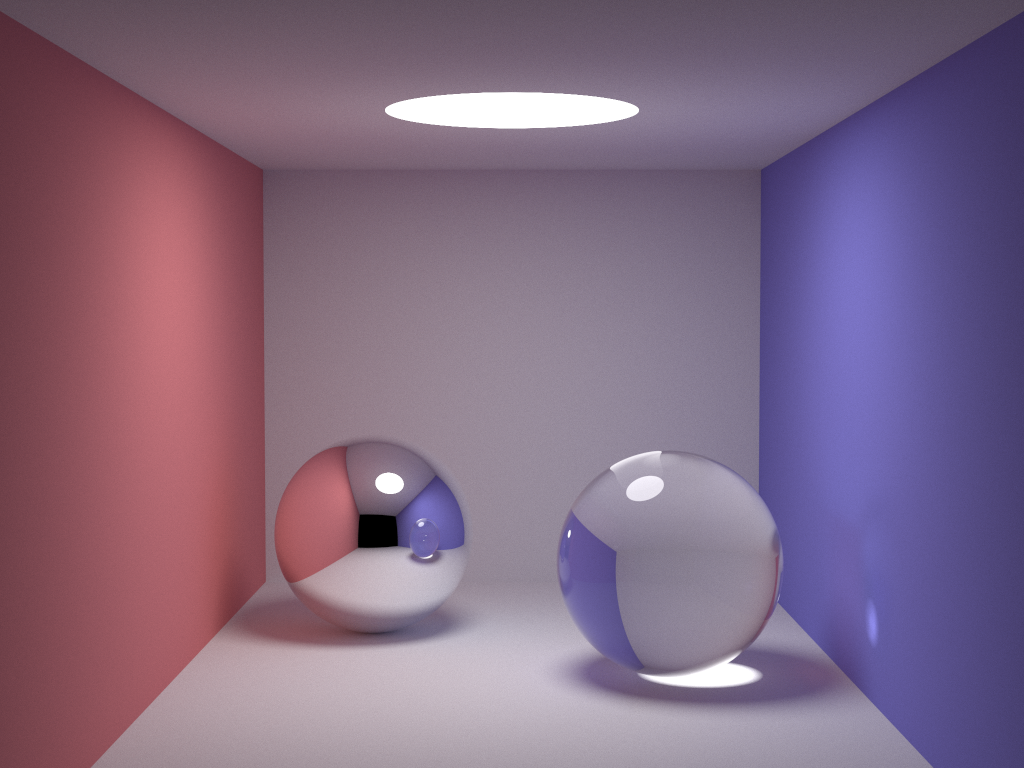
\includegraphics[height=0.8\textwidth]{./smallpt-render.png}
\end{column}
\begin{column}{0.48\textwidth}
\begin{itemize}
\item 99 LoC C++ raytracer.
\item Perfect for an optimization case study.
\item Ported to many languages, including Haskell! (Thanks to Vo Minh Thu(\texttt{noteed})).
\item Start from \texttt{noteed}'s original source; SHA the output image for baseline,
      keep optimizing.
\item Plan: Quick walk through Haskell code, end up at C++ (\texttt{clang++}) performance.
\end{itemize}
\end{column}
\end{columns}
\end{frame}

\note{Note for first slide: what is smallpt anyway?}

\begin{frame}[fragile]{What is smallpt anyway?}
% \begin{adjustwidth}{-5em}{-5em}
\begin{minted}{cpp}
struct Vec {      
  double x, y, z; // position, also color (r,g,b) 
  ... methods...
}; 
struct Ray { Vec o, d; Ray(Vec o_, Vec d_) : o(o_), d(d_) {} }; 
enum Refl_t { DIFF, SPEC, REFR };  // material types, used in radiance() 
struct Sphere { 
  double rad;   // radius 
  Vec p, e, c;  // position, emission, color 
  Refl_t refl;  // reflection type (DIFFuse, SPECular, REFRactive) 
  ... methods ...
  double intersect(const Ray &r) const // returns distance, 0 if nohit 
}; 
Sphere spheres[] = {//Scene: radius, position, emission, color, material 
  Sphere(1e5, Vec( 1e5+1,40.8,81.6), Vec(),Vec(.75,.25,.25),DIFF),//Left 
  ... initialization ...
}; 
\end{minted}
% \end{adjustwidth}
\end{frame}


\begin{frame}[fragile]{What is smallpt anyway?}
\footnotesize
\begin{minted}{cpp}
Vec radiance(const Ray &r, int depth, unsigned short *Xi){ 
                                                                         
                                                                         
                                                                      
                                                               
                                                                           
                                                                            
                                                                            
                                                                         
                                                                   
                                                                     
                                                                      
                                                           
                                                                          
                                                                            
                                                                            
                                                                           
                                                                        
                                                                          
                                                          
                                                                          
                                                                           
                                                                            
                                                                            
                                                                          
                                                                         
} 
\end{minted}
\end{frame}

\note{Say that the core function is radiance}

\begin{frame}[fragile]{What is smallpt anyway?}
\footnotesize
\begin{minted}{cpp}
Vec radiance(const Ray &r, int depth, unsigned short *Xi){ 
                                                                      
                                                                      
                                                                   
                                                            
                                                                        
                                                                         
                                       
                                          
                                                                
                                                                  
                                                                   
                          radiance
                                          
                          radiance
                                                                         
                                                                        
                                                                     
                                         
                          radiance
                                                                       
                                                                        
                                                                         
                                                                         
    radiance                      radiance
    radiance                      radiance
} 
\end{minted}
\end{frame}

\begin{frame}[fragile]{What is smallpt anyway?}

\note{Say that it's recursive}
\footnotesize
\begin{minted}{cpp}
Vec radiance(const Ray &r, int depth, unsigned short *Xi){ 
                                                                      
                                                                      
                                                                   
                                                            
                                                                        
                                                                         
  if (         ) if (             )            else 
  if (                ){                  
                                                                
                                                                  
                                                                   
                          radiance
  } else if (                )            
                          radiance
                                                                         
                                                                        
                                                                     
  if (                               )   
                          radiance
                                                                       
                                                                        
                                                                         
                                                                         
    radiance                      radiance
    radiance                      radiance
} 
\end{minted}
\end{frame}

\note{...with control flow}

\begin{frame}[fragile]{What is smallpt anyway?}
\footnotesize
\begin{minted}{cpp}
Vec radiance(const Ray &r, int depth, unsigned short *Xi){ 
                                                                      
                                                                      
                                                                   
                                                            
  Vec x=r.o+r.d*t, n=(x-obj.p).norm(), nl=n.dot(r.d)<0?n:n*-1, f=obj.c; 
                                                                         
  if (         ) if (             )            else 
  if (                ){                  
                                                                
                                                                  
                                                                   
                          radiance
  } else if (                )            
                          radiance
                                                                         
                                                                        
                                                                     
  if ((cos2t=1-nnt*nnt*(1-ddn*ddn))<0)
                          radiance
                                                                       
                                                                        
                                                                         
                                                                         
    radiance                      radiance
    radiance                      radiance
} 
\end{minted}
\end{frame}

\note{and lots of arithmetic}

\begin{frame}[fragile]{What is smallpt anyway?}
\footnotesize
\begin{minted}{cpp}
Vec radiance(const Ray &r, int depth, unsigned short *Xi){ 
  double t;                               // distance to intersection 
  int id=0;                               // id of intersected object 
  if (!intersect(r, t, id)) return Vec(); // if miss, return black 
  const Sphere &obj = spheres[id];        // the hit object 
  Vec x=r.o+r.d*t, n=(x-obj.p).norm(), nl=n.dot(r.d)<0?n:n*-1, f=obj.c; 
  double p = f.x>f.y && f.x>f.z ? f.x : f.y>f.z ? f.y : f.z; // max refl 
  if (++depth>5) if (erand48(Xi)<p) f=f*(1/p); else return obj.e; //R.R. 
  if (obj.refl == DIFF){                  // Ideal DIFFUSE reflection 
    double r1=2*M_PI*erand48(Xi), r2=erand48(Xi), r2s=sqrt(r2); 
    Vec w=nl, u=((fabs(w.x)>.1?Vec(0,1):Vec(1))%w).norm(), v=w%u; 
    Vec d = (u*cos(r1)*r2s + v*sin(r1)*r2s + w*sqrt(1-r2)).norm(); 
    return obj.e + f.mult(radiance(Ray(x,d),depth,Xi)); 
  } else if (obj.refl == SPEC)            // Ideal SPECULAR reflection 
    return obj.e + f.mult(radiance(Ray(x,r.d-n*2*n.dot(r.d)),depth,Xi)); 
  Ray reflRay(x, r.d-n*2*n.dot(r.d));     // Ideal dielectric REFRACTION 
  bool into = n.dot(nl)>0;                // Ray from outside going in? 
  double nc=1, nt=1.5, nnt=into?nc/nt:nt/nc, ddn=r.d.dot(nl), cos2t; 
  if ((cos2t=1-nnt*nnt*(1-ddn*ddn))<0)    // Total internal reflection 
    return obj.e + f.mult(radiance(reflRay,depth,Xi)); 
  Vec tdir = (r.d*nnt - n*((into?1:-1)*(ddn*nnt+sqrt(cos2t)))).norm(); 
  double a=nt-nc, b=nt+nc, R0=a*a/(b*b), c = 1-(into?-ddn:tdir.dot(n)); 
  double Re=R0+(1-R0)*c*c*c*c*c,Tr=1-Re,P=.25+.5*Re,RP=Re/P,TP=Tr/(1-P); 
  return obj.e + f.mult(depth>2 ? (erand48(Xi)<P ?   // Russian roulette 
    radiance(reflRay,depth,Xi)*RP:radiance(Ray(x,tdir),depth,Xi)*TP) : 
    radiance(reflRay,depth,Xi)*Re+radiance(Ray(x,tdir),depth,Xi)*Tr); 
} 
\end{minted}
\end{frame}

\note{display the whole thing}

\begin{frame}[fragile]{Initial Haskell Code: \texttt{radiance} ($1\times$)}
% 620027b45e40e5a4b18f36cabc70efe803f41a61
\begin{minted}[fontsize=\tiny]{hs}
radiance :: Ray -> CInt -> Ptr CUShort -> IO Vec
radiance ray@(Ray o d) depth xi = case intersects ray of
  (Nothing,_) -> return zerov
  (Just t,Sphere _r p e c refl) -> do
                                        
                                   
                                                              
                         
                                
        continue f = case refl of
          DIFF -> do
                                                
                               
                                
                                      
                                                                                           
                                  
                                                                                                                
                   radiance 
                                            
          SPEC -> do
                                                         
            rad <- radiance 
                                            
          REFR -> do
                                                                                                     
                                                                                   
                         
                           
                                                      
                                
                                                
            if 
              then do
                rad <- radiance reflRay depth' xi
\end{minted}

% \raw{Sha256} hash of the output image --- \raw{4dac691082bb}
\end{frame}

\note{show the same thing, this time in haskell}

\begin{frame}[fragile]{Initial Haskell Code: \texttt{radiance} ($1\times$) }
% 620027b45e40e5a4b18f36cabc70efe803f41a61
\begin{minted}[fontsize=\tiny]{hs}
radiance :: Ray -> CInt -> Ptr CUShort -> IO Vec
radiance ray@(Ray o d) depth xi = case intersects ray of
  (Nothing,_) -> return zerov
  (Just t,Sphere _r p e c refl) -> do
    let x = o `addv` (d `mulvs` t)
        n = norm $ x `subv` p
        nl = if n `dot` d < 0 then n else n `mulvs` (-1)
        pr = maxv c
        depth' = depth + 1
        continue f = case refl of
          DIFF -> do
            r1 <- ((2*pi)*) `fmap` erand48 xi
            r2 <- erand48 xi
            let r2s = sqrt r2
                w@(Vec wx _ _) = nl
                u = norm $ (if abs wx > 0.1 then (Vec 0 1 0) else (Vec 1 0 0)) `cross` w
                v = w `cross` u
                d' = norm $ (u`mulvs`(cos r1*r2s)) `addv` (v`mulvs`(sin r1*r2s)) `addv` (w`mulvs`sqrt (1-r2))
            rad <- radiance (Ray x d') depth' xi
            return $ e `addv` (f `mulv` rad)
          SPEC -> do
            let d' = d `subv` (n `mulvs` (2 * (n`dot`d)))
            rad <- radiance (Ray x d') depth' xi
            return $ e `addv` (f `mulv` rad)
          REFR -> do
            let reflRay = Ray x (d `subv` (n `mulvs` (2* n`dot`d)))
                into = n`dot`nl > 0                
                nc = 1
                nt = 1.5
                nnt = if into then nc/nt else nt/nc
                ddn= d`dot`nl
                cos2t = 1-nnt*nnt*(1-ddn*ddn)
            if cos2t<0
              then do
                rad <- radiance reflRay depth' xi
\end{minted}
% \raw{Sha256} hash of the output image --- \raw{4dac691082bb}
\end{frame}

\note{full code}


\begin{frame}[fragile]{Initial Haskell Code: Entry point  ($1\times$)}
\begin{minted}{hs}
smallpt :: Int -> Int -> Int -> IO ()
smallpt w h nsamps = do
  ...
  c <- VM.replicate (w * h) 0
  allocaArray 3 \xi -> -- Create mutable memory
    flip mapM_ [0..h-1] $ \y -> do -- Loop
      writeXi xi y
      for_ [0..w-1] \x -> do -- Loop
        let i = (h-y-1) * w + x
        for_ [0..1] \sy -> do -- Loop
          for_ [0..1] \sx -> do -- Loop
            r <- newIORef 0 -- Create mutable memory
            for_ [0..samps-1] \_s -> do -- Loops, Loops
              r1 <- (2*) <$> erand48 xi
              ...
              rad <- radiance (Ray (org+d.*140) (norm d)) 0 xi  -- Crunch
              ...
              modifyIORef r (+ rad .* recip (fromIntegral samps)) -- Write
            ci <- VM.unsafeRead c i
            Vec rr rg rb <- readIORef r
            VM.unsafeWrite c i $ 
                ci + Vec (clamp rr) (clamp rg) (clamp rb) .* 0.25 -- Write
\end{minted}
\end{frame}

\begin{frame}[fragile]{Initial Haskell Code: File I/O  ($1\times$)}
\begin{minted}{hs}
  withFile "image.ppm" WriteMode $ \hdl -> do
        hPrintf hdl "P3\n%d %d\n%d\n" w h (255::Int)
        flip mapM_ [0..w*h-1] \i -> do
          Vec r g b <- VM.unsafeRead c i
          hPrintf hdl "%d %d %d " (toInt r) (toInt g) (toInt b)
\end{minted}
\end{frame}

\begin{frame}[fragile]{Initial Haskell Code: RNG ($1\times$)}
\begin{minted}{hs}
foreign import ccall unsafe "erand48"
  erand48 :: Ptr CUShort -> IO Double
\end{minted}
\end{frame}


\begin{frame}[fragile]{Restrict export list to `main` ($1.13\times$)}
% 4678326cbb78368977f901ed32e0bdb55b8be6c7
\begin{minted}{diff}
-module Main where
+module Main (main) where
\end{minted}

\pause
\begin{itemize}
\item Exported functions could be used by something unknown.
\item original versions must be available. \pause
\item Make many optimizations unsound.
\end{itemize}
\end{frame}

\note{
The very first thing to do is to let the compiler actually optimize.  Exported
functions could be used by something unknown to the compiler and thus their
original versions must be available. This makes many optimizations look bad or
be unreasonable. Explicit export lists tell the compiler what you care about.
They aren't just about encapsulation.
}

\begin{frame}[fragile]{Mark entries of Ray and Sphere as UNPACK and Strict ($1.07\times$)}
% 1ad231a927f1a0582aee3f161e91372f7124d0c7

\begin{minted}[fontsize=\small]{diff}
data Vec = Vec {-# UNPACK #-} !Double 
               {-# UNPACK #-} !Double 
               {-# UNPACK #-} !Double

-data Ray = Ray Vec Vec -- origin, direction
+data Ray = Ray {-# UNPACK #-} !Vec {-# UNPACK #-} !Vec -- origin, direction

 data Refl = DIFF | SPEC | REFR -- material types, used in radiance

 -- radius, position, emission, color, reflection
-data Sphere = Sphere Double Vec Vec Vec !Refl
+data Sphere = Sphere {-# UNPACK #-} !Double 
+                     {-# UNPACK #-} !Vec 
+                     {-# UNPACK #-} !Vec 
+                     {-# UNPACK #-} !Vec !Refl
\end{minted}

\begin{minted}[fontsize=\small]{cpp}
struct Vec { double x, y, z; }
struct Ray { std::function<Vec()> v; std::function<Vec()> w; };
struct RayUnpack { double xv, yv, int zv;
                   double xw, yw, zw; };
\end{minted}
\end{frame}

\note{ Strict means that they're evaluated ahead of time, not lazily of course.
This can save a bit in their evaluation cost but means we always pay it. It is
a trade off but here we know it will be a good one because we have almost
perfect demand.  Unpacking is different. It removes indirection of doing a
memory lookup for components but means we have to copy everything into the data
structure that it is unpacked into.  We don't unpack ray because we'll be doing
a lot of calculations on it and we want the Vec math to fuse and not get
copied, when we use the Vecs they should be hot in cache anyway.  We do inline
Sphere because we statically create them and while they'll also be hot in cache
there is no benefit to taking any extra cost at all.
}


\begin{frame}[fragile]{Use a pattern synonym to unpack Refl in Sphere ($1.07\times$)}
% e1819a6

\begin{minted}[fontsize=\small]{diff}
+{-# LANGUAGE PatternSynonyms #-}
\end{minted}


\begin{minted}[fontsize=\small]{diff}
-data Refl = DIFF | SPEC | REFR -- material types, used in radiance
+newtype Refl = Refl Int  -- material types, used in radiance
+pattern DIFF,SPEC,REFR :: Refl
+pattern DIFF = Refl 0
+pattern SPEC = Refl 1
+pattern REFR = Refl 2
+{-# COMPLETE DIFF, SPEC, REFR #-}

 -- radius, position, emission, color, reflection
 data Sphere = Sphere {-# UNPACK #-} !Double 
                      {-# UNPACK #-} !Vec
                      {-# UNPACK #-} !Vec 
-                     {-# UNPACK #-} !Vec !Refl
+                     {-# UNPACK #-} !Vec {-# UNPACK #-} !Refl

 \end{minted}

\end{frame}

\note{
Until the recent addition of unboxed sums in GHC there was no way to unpack a type with multiple constructors.
While unboxed sums exist now, their syntax is quite unpleasant.
We're using an older trick to fake the unboxing here instead.
In this case it isn't much of a win, but it illustrates the technique.
}


\begin{frame}[fragile]{Change from \texttt{maximum} on a list to \texttt{max} ($1.08\times$)}
% e77b26f
\begin{minted}{diff}
-maxv (Vec a b c) = maximum [a,b,c]
+maxv (Vec a b c) = max a (max b c)
\end{minted}

\begin{minted}{diff}
     let x = o `addv` (d `mulvs` t)
         n = norm $ x `subv` p
         nl = if n `dot` d < 0 then n else n `mulvs` (-1)
-        pr = maxv c
         depth' = depth + 1
         continue f = case refl of
           DIFF -> do
...
     if depth'>5
       then do
         er <- erand48 xi
+        let !pr = maxv c
\end{minted}
\end{frame}

\note{finicky optimization. GHC does not evaluate at compile time, making
      optimizations like these necessary}


\begin{frame}[fragile]{Convert \texttt{erand48} to pure Haskell ($1.09\times$)}
% 48aeb46
\begin{minted}[fontsize=\small]{diff}
-radiance :: Ray -> CInt -> Ptr CUShort -> IO Vec
+radiance :: Ray -> Int -> IORef Word64 -> IO Vec
 radiance ray@(Ray o d) depth xi = case intersects ray of
   (Nothing,_) -> return zerov
   (Just t,Sphere _r p e c refl) -> do
@@ -153,9 +153,8 @@ smallpt w h nsamps = do
       cx = Vec (fromIntegral w * 0.5135 / fromIntegral h) 0 0
       cy = norm (cx `cross` dir) `mulvs` 0.5135
   c <- VM.replicate (w * h) zerov
-  allocaArray 3 $ \xi ->
-      flip mapM_ [0..h-1] $ \y -> do
+  xi <- newIORef 0
+  flip mapM_ [0..h-1] $ \y -> do
       writeXi xi y
\end{minted}
\end{frame}

\note{
This function isn't used much so it doesn't really impact our performance but
often building unnecessary data structures is detrimental.
}

\begin{frame}[fragile]{Remove mutability: \texttt{Erand48} Monad}


\begin{minted}[fontsize=\small]{diff}
-erand48 :: IORef Word64 -> IO Double
-erand48 !t =  do
-  r <- readIORef t
+data ET a = ET !Word64 !a deriving Functor
+newtype Erand48 a = Erand48 { runErand48' :: Word64 -> ET a } deriving Functor
+instance Applicative Erand48 where
+instance Monad Erand48 where
+runWithErand48 :: Int -> Erand48 a -> a                                                                                                
+erand48 :: Erand48 Double
...
-radiance :: Ray -> Int -> IORef Word64 -> IO Vec
-radiance ray@(Ray o d) depth xi = case intersects ray of
+radiance :: Ray -> Int -> Erand48 Vec
+radiance ray@(Ray o d) depth = case intersects ray of
...
-            r1 <- (2*pi*) <$> erand48 xi
-            r2 <- erand48 xi
+            r1 <- (2*pi*) <$> erand48
+            r2 <- erand48
...
-                              then (.* rp) <$> radiance reflRay depth' xi
-                              else (.* tp) <$> radiance (Ray x tdir) depth' xi
+                              then (.* rp) <$> radiance reflRay depth'
+                              else (.* tp) <$> radiance (Ray x tdir) depth'
\end{minted}
\end{frame}

\note{
The entire premise of this talk is that Haskell can be as fast as C.  Further
any impedance mismatch, such as FFI almost universally has to have, carries
some bookkeeping overhead. If our Haskell code was as fast as the C code moving
the code into Haskell would be a win, if it was slightly slower it could still
be a win.  Often considering your Haskell code's performance is a better option
and easier than reimplementing something in C.
As is the way with optimizations, this is not universally true.
}

\begin{frame}[fragile]{Removing mutation: eliminate \texttt{IORef}}
\begin{minted}[fontsize=\small]{diff}
-  c <- VM.replicate (w * h) 0
-  xi <- newIORef 0
-  flip mapM_ [0..h-1] $ \y -> do
-      writeXi xi y
-      for_ [0..w-1] \x -> do
-        let i = (h-y-1) * w + x
-        for_ [0..1] \sy -> do
-          for_ [0..1] \sx -> do
-            r <- newIORef 0
-            for_ [0..samps-1] \_s -> do
-              r1 <- (2*) <$> erand48 xi
+      img = (`concatMap` [(h-1),(h-2)..0]) $ \y -> runWithErand48 y do
+        for [0..w-1] \x -> do
+          (\pf -> foldlM pf 0 [(sy, sx) | sy <- [0,1], sx <- [0,1]]) \ci (sy, sx) -> do
+            Vec rr rg rb <- (\f -> foldlM f 0 [0..samps-1]) \ !r _s -> do
+              r1 <- (2*) <$> erand48
...
-              modifyIORef r (+ rad .* recip (fromIntegral samps))
-            ci <- VM.unsafeRead c i
-            Vec rr rg rb <- readIORef r
-            VM.unsafeWrite c i $ ci + Vec (clamp rr) (clamp rg) (clamp rb) .* 0.25
+              pure (r + rad .* recip (fromIntegral samps))
+            pure (ci + Vec (clamp rr) (clamp rg) (clamp rb) .* 0.25)
...
\end{minted}
\end{frame}


\note{
All these mutability locations throw in extra RTS code, extra sequencing that
blocks the compiler's optimization, and dependency chains.  
Sometimes we need
mutability for performance but in fact one primary optimization technique
powering modern compilers is SSA. We almost start there as a functional
language don't break it when you don't have a good reason.
}


\begin{frame}[fragile]{Set \textbf{everything} in \texttt{smallpt} to be strict ($1.17\times$)}
% e62177b
\begin{minted}[fontsize=\small]{diff}
smallpt :: Int -> Int -> Int -> IO ()
smallpt w h nsamps = do
-  let samps = nsamps `div` 4
-      org = Vec 50 52 295.6
-      dir = norm $ Vec 0 (-0.042612) (-1)
-      cx = Vec (fromIntegral w * 0.5135 / fromIntegral h) 0 0
-      cy = norm (cx `cross` dir) `mulvs` 0.5135
+  let !samps = nsamps `div` 4
+      !org = Vec 50 52 295.6
+      !dir = norm $ Vec 0 (-0.042612) (-1)
+      !cx = Vec (fromIntegral w * 0.5135 / fromIntegral h) 0 0
+      !cy = norm (cx `cross` dir) `mulvs` 0.5135
...
-  r1 <- (2*) `fmap` erand48 xi
-  let dx = if r1<1 then sqrt r1-1 else 1-sqrt(2-r1)
-  r2 <- (2*) `fmap` erand48 xi
-  let dy = if r2<1 then sqrt r2-1 else 1-sqrt(2-r2)
-      d = ...
-  rad <- radiance (Ray (org`addv`(d`mulvs`140)) (norm d)) 0 xi
+  !r1 <- (2*) `fmap` erand48 xi
+  let !dx = if r1<1 then sqrt r1-1 else 1-sqrt(2-r1)
+  !r2 <- (2*) `fmap` erand48 xi
+  let !dy = if r2<1 then sqrt r2-1 else 1-sqrt(2-r2)
+      !d = ...
...
+              pure $! r + rad .* recip (fromIntegral samps)
+            pure $! ci + Vec (clamp rr) (clamp rg) (clamp rb) .* 0.25
\end{minted}
\end{frame}

\note{
This is not a recommendation, this is a warning.
We get a speedup here but it can also regress performance. Some of these bangs are regressions that are hidden.
Don't senselessly bang everything in sight.
}

\begin{frame}[fragile]{Why strictness may be bad}
\begin{minted}[fontsize=\small]{hs}
let foo = let x = error "ERR" in \y -> y
let foo' = let !x = error "ERR" in \y -> y
\end{minted}
\pause
\begin{minted}[fontsize=\small]{hs}
let fooOpt = \y -> y
let foo'Opt = \y -> y  -- ERROR! forcing foo' should give "ERR"
\end{minted}
\pause
\begin{minted}[fontsize=\small]{hs}
let tuple = (42, error "urk")
let bar = let (x, y) = tuple in \z -> x + z
\end{minted}
\pause
\begin{minted}[fontsize=\small]{hs}
let barOpt = \z -> 42 + z
\end{minted}
\pause
\begin{minted}[fontsize=\small]{hs}
let bar' = let (x, !y) = tuple in \z -> x + z
\end{minted}
\pause
\begin{minted}[fontsize=\small]{hs}
let bar'Opt =  \z -> 42 + z  --  ERROR: forcing bar' should give "urk"
\end{minted}
\end{frame}


\begin{frame}[fragile]{Reduce to only useful strictnesses in \texttt{smallpt}($1.17\times$)}
\begin{minted}{diff}
-  let !samps = nsamps `div` 4
-      !org = Vec 50 52 295.6
-      !dir = norm $ Vec 0 (-0.042612) (-1)
-      !cx = Vec (fromIntegral w * 0.5135 / fromIntegral h) 0 0
-      !cy = norm (cx `cross` dir) .* 0.5135
+  let samps = nsamps `div` 4
+      org = Vec 50 52 295.6
+      dir = norm $ Vec 0 (-0.042612) (-1)
+      cx = Vec (fromIntegral w * 0.5135 / fromIntegral h) 0 0
+      cy = norm (cx `cross` dir) .* 0.5135
...
-              !r1 <- (2*) <$> erand48
+              r1 <- (2*) <$> erand48
...
-              !r2 <- (2*) <$> erand48
+              r2 <- (2*) <$> erand48
...
-              !rad <- radiance (Ray (org+d.*140) (norm d)) 0
+              rad <- radiance (Ray (org+d.*140) (norm d)) 0
...
-              pure $! r + rad .* recip (fromIntegral samps)
-            pure $! ci + Vec (clamp rr) (clamp rg) (clamp rb) .* 0.25
+              pure (r + rad .* recip (fromIntegral samps))
+            pure (ci + Vec (clamp rr) (clamp rg) (clamp rb) .* 0.25)
\end{minted}
\end{frame}

\note{
Bangs force evaluation.
The computation might diverge.
Thus the compiler can no longer move the computation around or simplify it.
Also if the work doesn't have to get done it still might be.
A little thinking about how the variables are used or looking at core allows us to select which ones we bang selectively.
}

\begin{frame}[fragile]{Use strictness strategically in entire project}
\begin{minted}[fontsize=\small]{diff}
...
-  if det<0 then Nothing else f (b-sdet) (b+sdet)
-  where op = p - o
-        eps = 1e-4
-        b = dot op d
-        det = b*b - dot op op + r*r
-        sdet = sqrt det
-        f a s = if a>eps then Just a else if s>eps then Just s else Nothing
+  if det<0
+  then Nothing
+  else
+    let !eps = 1e-4
+        !sdet = sqrt det
+        !a = b-sdet
+        !s = b+sdet
+    in if a>eps then Just a else if s>eps then Just s else Nothing
...
\end{minted}
\end{frame}

\note{
Sometimes (point out 'intersect') we have to rearrange the code though when we use bangs.
Bangs tell the compiler to make more efficient code, but take away the compiler's options in how to do so. Only take away the compiler's liberties when it's using them poorly.
After a little trial and error or reading core how to use bangs in your code will be intuitive.
}


\begin{frame}[fragile]{Remove \texttt{Maybe} from \texttt{intersect(s)} ($1.32\times$)}
% 09f43c7
\begin{minted}[fontsize=\small]{diff}
| Old: Use Maybe Double to represent (was-hit?:bool, hit-distance: Double)
| New: use (1/0) to represent not (was-hit?)
-intersect :: Ray -> Sphere -> Maybe Double
+intersect :: Ray -> Sphere -> Double
intersect (Ray o d) (Sphere r p _e _c _refl) =
-  if det<0 then Nothing else f (b-sdet) (b+sdet)
+  if det<0 then (1/0.0) else f (b-sdet) (b+sdet)
   where op = p `subv` o
         ...
-        f a s = if a>eps then Just a else if s>eps then Just s else Nothing
+        f a s = if a>eps then a else if s>eps then s else (1/0.0)

-intersects :: Ray -> (Maybe Double, Sphere)
+intersects :: Ray -> (Double, Sphere)
 intersects ray = (k, s)
-  where (k,s) = foldl' f (Nothing,undefined) spheres
-        f (k',sp) s' = case (k',intersect ray s') of
-                  (Nothing,Just x) -> (Just x,s')
-                  (Just y,Just x) | x < y -> (Just x,s')
-                  _ -> (k',sp)
+  where (k,s) = foldl' f (1/0.0,undefined) spheres
+        f (k', sp) s' = let !x = intersect ray s' in if x < k' then (x, s') else (k', sp)
 
 radiance :: Ray -> Int -> STRefU s Word64 -> ST s Vec
 radiance ray@(Ray o d) depth xi = case intersects ray of
-  (Nothing,_) -> return zerov
-  (Just t,Sphere _r p e c refl) -> do
+  (t,_) | t == (1/0.0) -> return zerov
+  (t,Sphere _r p e c refl) -> do
\end{minted}
\end{frame}

\note{
    This is a far more performance critical version of what we saw with 'maximum' vs. 'max'.

    Our innermost functions are of critical importance. Here we remove
    a Maybe which significantly reduces the boxing (which could have
    been mitigated with a StrictMaybe) and the cases.

    Since a Ray that fails to intersect something can be said to
    intersect at infinity, Double already actually covers the
    structure at play.

    This also reduces allocation.}

\begin{frame}[fragile]{Hand unroll the fold in intersects ($1.35\times$)}
% 4f28fcc

\begin{minted}[fontsize=\small]{diff}
intersects :: Ray -> (Double, Sphere)
-intersects ray = (k, s)
-  where (k,s) = foldl' f (1/0.0,undefined) spheres
+intersects ray =
+    f (... (f (f (intersect ray sphLeft, sphLeft) sphRight) ...)
+  where
     f (k', sp) s' = let !x = intersect ray s' in if x < k' then (x, s') else (k', sp)
\end{minted}

\note{
Sadly 'intersects' remains one of our most costly functions even after that improvement so we'll focus on it a bit.
A common optimization is loop unrolling.
Many compilers do this for us, and there are special versions of it like Duff's Device.
Sadly GHC is the one compiler I've used that doesn't.
We can though implement every variety of it I know of by hand in Haskell, and this is one of the simplest.
I believe we could produce a rule that did it for a given function but I've not actually explored that.
}

\begin{minted}[fontsize=\small]{diff}
-spheres :: [Sphere]
-spheres = let s = Sphere ; z = zerov ; (.*) = mulvs ; v = Vec in
-  [ s 1e5 (v (1e5+1) 40.8 81.6)    z (v 0.75 0.25 0.25) DIFF --Left
-  , s 1e5 (v (-1e5+99) 40.8 81.6)  z (v 0.25 0.25 0.75) DIFF --Rght
...

+sphLeft, sphRight, ...  :: Sphere
+sphLeft  = Sphere 1e5  (Vec (1e5+1) 40.8 81.6)    zerov (Vec 0.75 0.25 0.25) DIFF
+sphRight = Sphere 1e5  (Vec (-1e5+99) 40.8 81.6)  zerov (Vec 0.25 0.25 0.75) DIFF
...
\end{minted}

\end{frame}

\begin{frame}[fragile]{Custom datatype for \texttt{intersects} parameter passing}
\begin{minted}{diff}
Old: Tuple with possibly-uenevaluated Double and Sphere
New: Reference to a guaranteed-to-be-evaluated Double and Sphere
-intersects :: Ray -> (Double, Sphere)
+data T = T !Double !Sphere 
+
+intersects :: Ray -> T
 intersects ray =
-    f ( ... f (intersect ray sphLeft, sphLeft) sphRight) ... sphLite
+    f ( ... f (T (intersect ray sphLeft) sphLeft) sphRight) ... sphLite
   where
-    f (k', sp) s' = 
-        let !x = intersect ray s' in if x < k' then (x, s') else (k', sp)
+    f !(T k' sp) !s' =
+        let !x = intersect ray s' in if x < k' then T x s' else T k' sp
 
 radiance :: Ray -> Int -> Erand48 Vec
 radiance ray@(Ray o d) depth = case intersects ray of
-  (!t,_) | t == 1/0.0 -> return 0
-  (!t,!Sphere _r p e c refl) -> do
+  (T t _) | t == 1/0.0 -> return 0
+  (T t (Sphere _r p e c refl)) -> do
     let !x = o + d .* t
         !n = norm $ x - p
         !nl = if dot n d < 0 then n else negate n
\end{minted}
\end{frame}

\note{
Still trying to focus on the performance of 'intersects' we can optimize how it passes data to itself and its caller.
We want the data to be strict so the compiler knows the tuple's members will always be evaluated, but we want to avoid copying.
A normal tuple lacks strictness information.
An unboxed tuple sadly forces copying because of its unpacked nature. Sphere is quite large, and will be expensive to copy.
What we need is a strict tuple, and we create one for just this usage.
This exists in libraries of course, but we wanted to illustrate it.
}

\begin{frame}[fragile]{Optimize file writing}
\begin{minted}{diff}
   build-depends:
       base >= 4.12 && < 4.15
+    , bytestring ^>= 0.11
\end{minted}
\begin{minted}{diff}
-toInt :: Double -> Int
-toInt x = floor $ clamp x ** recip 2.2 * 255 + 0.5
+toInt :: Double -> BB.Builder -- O(1) concatenation
+toInt x = BB.intDec (floor (clamp x ** recip 2.2 * 255 + 0.5)) <> BB.char8 ' '
... 
   withFile "image.ppm" WriteMode $ \hdl -> do
-        hPrintf hdl "P3\n%d %d\n%d\n" w h (255::Int)
-        for_ img \(Vec r g b) -> do
-          hPrintf hdl "%d %d %d " (toInt r) (toInt g) (toInt b)
+        BB.hPutBuilder hdl $
+          BB.string8 "P3\n" <>  -- efficient builders for ASCII
+          BB.intDec w <> BB.char8 ' ' <> BB.intDec h <> BB.char8 '\n' <>
+          BB.intDec 255 <> BB.char8 '\n' <>
+          (mconcat $ fmap (\(Vec r g b) -> toInt r <> toInt g <> toInt b) img)
\end{minted}
\end{frame}

\note{
We're getting quite a bit faster now, but there's still some small pieces of low lying fruit.
Strings are fairly inefficient and the conversion functions to them we use aren't particularly efficient.
'bytestring' has some efficient writing code, so we just convert to that for a modest gain. 
}


\begin{frame}[fragile]{Use \texttt{LLVM} backend ($1.87\times$)}
% 578b83c0afb6a8c7944529e2607ef9dbd5f2ab22
\begin{minted}{diff}
+package smallpt-opt 
+  ghc-options: -fllvm
\end{minted}
\end{frame}

\note{
Finally, this particular code is quite numeric heavy.
There are optimizations for numeric heavy code we're missing in GHC.
LLVM has an extensive library of laws to optimize low level numeric ops. 
LLVM is too low-level to understand haskell as haskell. It makes decisions with the tacit assumption that the assembly came from a C-like language, which is often to the detriment of a Haskell-like language.
In this case, as the code is “fortran-like”, LLVM wins.
}

\begin{frame}[fragile]{The view from the mountaintop}

\begin{center}
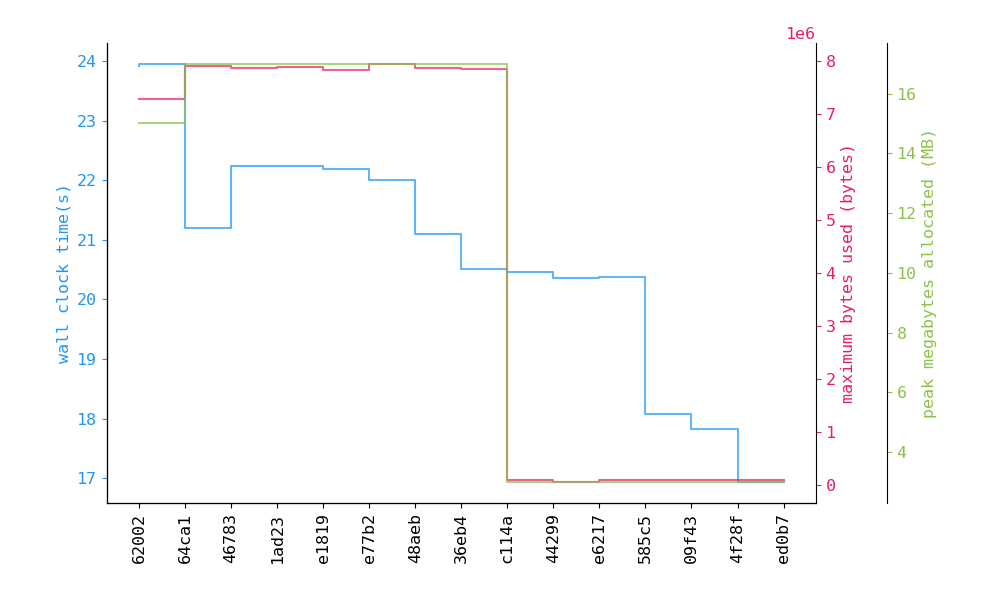
\includegraphics[height=0.6\textwidth]{./perfdata-gen.png}
\end{center}

%{\tiny
%\begin{minted}{text}
%64ca171 Replace CDouble with Double because its just a newtype.
%4678326 Restrict the export list to 'main'.
%1ad231a Mark entries of Ray and Sphere as UNPACK and Strict.
%e1819a6 Use a pattern synonym to unpack Refl in Sphere.
%e77b26f Change from maximum on a list to max.
%48aeb46 Convert erand48 to pure Haskell.
%36eb49e Change erand48 to IORefU.
%c114ace Rewrite the remaining IORef into a foldM.
%44299aa Remove the Data.Vector.Mutable by being purer.
%e62177b Set everything in smallpt to be strict.
%585c5cb Reduce to only effectful strictnesses.
%09f43c7 Remove Maybe from intersect(s)
%4f28fcc Hand unroll the fold in intersects.
%ed0b794 Marking interesects' f parameters strict.
%8309e4a Strategic application of strictness.
%7be5b4b Shorted erand48.
%578b83c Use LLVM backend.
%\end{minted}
%}
\end{frame}


\begin{frame}[fragile]{Takeaways}
\begin{itemize}
\item The unrolling in 'intersects' is ugly.
\item (We feel) the maintainability of this code hasn’t been significantly harmed.
\item We're faster than clang++ and within 6\% of g++
\item Haven't exhausted the optimization opportunities.
\item GHC could learn to do several of these optimizations for us.
\item Others are just good Haskell style. 
\item Clean Haskell is often performant Haskell.
\end{itemize}
%\item \href{https://docs.google.com/spreadsheets/d/1YhZlDRGvnCtN8UQf_0ItmgRWI9MhL21HDTlBEKqgWHc/edit#gid=0}{Raw Google Sheet of our transformations}
%\item \href{https://github.com/bollu/smallpths}{\texttt{github.com/bollu/smallpt-opt}}
\end{frame}

\note{
The unrolling in 'intersects' is ugly but other than that optimization it is our opinion that the maintainability of this code hasn’t been significantly harmed by improving its performance.
We're faster than clang++ and within 6% of g++, we're closer to g++ than clang++.
We haven't exhausted the optimization opportunities.
I believe GHC could learn to do several of these optimizations for us.
Many of the others are just good Haskell style.
Clean Haskell is often performant Haskell.
}
\end{document}
